\documentclass[varwidth=true, border=2pt]{standalone}

\usepackage{tikz}
\usetikzlibrary{shapes.misc}

\begin{document}
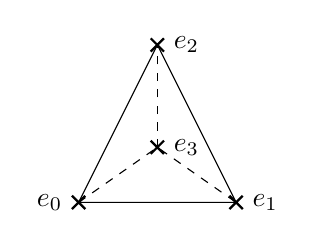
\begin{tikzpicture}
    \tikzstyle{point}=[thick,draw=black,cross out,inner sep=0pt,minimum width=4pt,minimum height=4pt]

    \node (a)[point,label={[label distance=0cm]180:$e_0$}] at (0,0) {};
    \node (b)[point,label={[label distance=0cm]0:$e_1$}] at (2,0) {};
    \node (c)[point,label={[label distance=0cm]0:$e_2$}] at (1,2) {};
    \node (d)[point,label={[label distance=0cm]0:$e_3$}] at (1,0.7) {};
    \draw (a.center) -- (b.center) -- (c.center) -- cycle;
    \draw[dashed] (a.center) -- (d.center) -- (b.center);
    \draw[dashed] (d.center) -- (c.center);
\end{tikzpicture}
\end{document}
